\documentclass[oneside]{book}

%\usepackage{tipa}
\usepackage{multicol}
\usepackage{tablefootnote,tipa}

%\usepackage{gb4e}


\usepackage{tikz}
\usetikzlibrary{shapes.geometric}

\usepackage{gb4e}

\usepackage{hyperref}
\usepackage{multirow}

\usepackage{lscape}

\newcommand{\ti}{\textipa}

\begin{document}
\tableofcontents



\part{Morphology}
\chapter{Nominals}
\section{Overview}

Loric is a synthetic, fusional language --- much of its inspiration comes from Latin, its modern Romance daughter languages, and Attic Greek, all of which are to some degree inflectional. As would be expected from these influences, Loric is highly inflected. The following table shows which parts of speech must be marked morphologically to denote number, case, or gender:

{
\begin{center}
    \begin{tikzpicture}
    \node[regular polygon, regular polygon sides = 3, minimum size = 6.5cm] (p) at (0,0) {};
    \node[regular polygon, regular polygon sides = 3, minimum size = 4.5cm, draw] (q) at (0,0) {};
     \node[regular polygon, regular polygon sides = 3, minimum size = 7cm] (r) at (0,0) {};


     \node[regular polygon, regular polygon sides = 3, minimum size = 9cm] (s) at (0,0) {};

    \node[] at (p.90) {\textbf{Number}};

    \node[] at (p.210) {\textbf{Case}};
    \node[] at (p.330) {\textbf{Gender}};

     \node[] at (r.150) {Nouns};
     \node[] at (r.270) {Adjectives};
     \node[align = left, text width = 2cm] at (s.390) {Pronouns, Articles};






    \end{tikzpicture}
\end{center}
}
As can be seen, while no word obligatorily marks \textit{all} these factors, they all must mark at least two, This means that there is generally enough redundancy in marking features to permit the hallmark advantages of an inflected language - pro-drop and free(ish) word order.


\section{Noun Class (`Gender'`)}

Loric's noun class system is somewhere between a European-style gender system and an animacy hierarchy. The four classes are:

\begin{itemize}
    \item Exalted (E)
    \begin{itemize}
        \item Gods and deities (of state-approved religions), monarchs, official titles and offices, historical figures held in high esteem, some place names, most weapons and tools for combat. Anything with religious or ceremonial function.
    \end{itemize}
    \item Civilized (C)
    \begin{itemize}
        \item The majority of job titles and proper names, agricultural and artisan tools,  some domestic animals. Things made by humans (foods, works of art, buildings, etc)  Abstract concepts and emotions that are not explicitly to be avoided (love, honor)  This also functions as a ``miscellaneous'' category for loanwords and neologisms.
    \end{itemize}
    \item Wild (W)
    \begin{itemize}
        \item Most animals, natural features (mountains, forests, etc), plants, animate nonliving things (fire, air),  astronomical bodies (except the sun, which is Exalted)
    \end{itemize}
    \item Accursed (A)
    \begin{itemize}
        \item Dangerous animals, poisonous plants, inhospitable terrain (deserts, bogs), diseases, curses, negative emotions, machines.
    \end{itemize}
\end{itemize}


This taxonomy should be considered at best some rough rules of thumb for determining a noun's class --- exceptions abound. \\

\newpage
\section{Case Endings}
\label{section:cases}
Nouns are obligatorily marked for case and number, using the below endings. Note that often the quality of vowels in case endings is dependant on the stem word; the \$ symbol is used to indicate a ``null vowel'' that assimilates to the rightmost vowel in the stem. For example:

\smallskip
\begin{exe}
\ex \textit{ranje} ``fruit'' + accusative singular ending --l\$ $\rightarrow$ \textit{ranjele}
\end{exe}
\begin{center}
\begin{tabular}{c| c c c}
  & \textbf{Sg} & \textbf{Pc} & \textbf{Pl} \\
  \hline
\textbf{NOM} & --\O & --ll\$ & --\O\textipa{:} \\
\textbf{ACC} & --l\$ & --ll\$ & --l\$n \\
\textbf{GEN} & --j & --j\$ll\$ & --j\$n \\
\textbf{LOC} & --t & --d\$ll\$  &--d\$n \\
\textbf{ABL} & --x & --ll\$x & --x\$n \\
\textbf{ALL} & --z & --ll\$z & --z\$n \\
\textbf{INS} & --r & --ll\$r & --r\$n \\
\textbf{VOC} & --k & \multicolumn{2}{c}{--k\$la} \\


\end{tabular}

\end{center}
For the nominative plural form, the final vowel is lengthened and no affixes are added:


\begin{exe}
\ex \textit{kani} ``dog'' $\rightarrow$ \textit{kan\ti{\=i}} (\textipa{kA.ni:}) ``many dogs''
\end{exe}

Also worth pointing out is the \textit{ll} sequence present in all paucal forms except the vocative; this is a remnent of the paucal's previous function in Old High Loric as a dual marker, based on the word \textit{alla} ``two.''
\section{Articles}
Much like in Arabic, a definite article is required to preceed a noun in nearly all cases. The definite article is marked for gender and number:

\begin{center}
\begin{tabular}{c| c c c }
& \textbf{Sg} & \textbf{Pc} & \textbf{Pl} \\
\hline
\textbf{C1} & re & rex & ren \\
\textbf{C2} & ye & yeve & yen \\
\textbf{C3} & xi & xe & xen \\
\textbf{C4} & pse & psen & ox
\end{tabular}
\end{center}

When the article form ends with a vowel and the following noun begins with a vowel, the article vowel is elided and the article becomes affixed as a clitic:


\begin{exe}
  \ex ye kisi ``the person''
  \ex y'a\ti{\.*na} ``the paper''
\end{exe}

\section{Pronouns} 
\bigskip
\begin{minipage}[c]{.5\textwidth}

\centering

\textbf{Personal Pronouns} \\
\medskip
\begin{tabular}{c| c c c }
& \textbf{Sg} & \textbf{Pc} & \textbf{Pl} \\
\hline
\textbf{1p} & ejeqe & xreqe & osmiqi \\
\textbf{2p} & e\ti{\.*m}eqe  & e\ti{\.*l}eqe & i\ti{\.*l}iqi \\
\textbf{3p} & voqo & hoqo & axriqi 

\end{tabular}

\end{minipage}
\begin{minipage}[c]{.5\textwidth}
\centering

\textbf{Reflexive Pronouns} \\
\medskip

\begin{tabular}{c| c c c }
& \textbf{Sg} & \textbf{Pc} & \textbf{Pl} \\
\hline
\textbf{1p} & eje & xre & osmi \\
\textbf{2p} & e\ti{\.*m}e  & e\ti{\.*l}e & i\ti{\.*l}i \\
\textbf{3p} & vox & ho & axri 

\end{tabular}

\end{minipage}

\bigskip



\newpage




\chapter{Verbs}
\section{Overview of Verbs}




The primary ways a verb changes form is to mark \textit{subject number, tense, aspect,} and \textit{mood.} Subject number and aspect marking and are handled by suffixes, while all other changes are encoded as changes to the verbal stem.




\section{Subject Affixes}

Much like was seen for case (see \ref{section:cases}), verbal subject endings often mutate to match the rightmost vowel in the stem. Also note that there is no distinction between the paucal and the plural in verb morphology; both are marked with the plural set of endings.

\subsection{The Aorist Endings}

The present subject affixes are used to denote a present aorist aspect, without reference to the ``completeness'' of the action:\footnote{Again, that \textit{ll} sequence shows up here. Similar to the paucal case endings, (see \ref{section:cases}), this reflects an etymological connection with \textit{alla}, ``two,'' this time going back to the Archaic/Early High period use to mean ``other,'' functioning as an informal second person pronoun}

\begin{center}

\begin{tabular}{c| c c }
  & \textbf{Sg} & \textbf{Pc/Pl} \\
  \hline
  \textbf{1p} & --n & --m \\
  \textbf{2p}& --ll\$ & --ll\$m \\
  \textbf{3p} & --\O & --v\$m

\end{tabular}

\end{center}


%TODO examples

\subsection{The Perfective Endings}
Aspect is marked by the use of alternate verb endings:

For the perfective aspect, the endings are:
\begin{center}
\begin{tabular}{c| c c }
  & \textbf{Sg} & \textbf{Pc/Pl} \\
  \hline
  \textbf{1p} & --n\$ & --n\$\textipa{:}ri \\
  \textbf{2p} & --ll\$ & --ll\$m \\
  \textbf{3p} & --\O & --n\$m

\end{tabular}
\end{center}

Note that in general, since the perfective stem ends in a geminate consonant (see \ref{section:perfstem}), adding perfective endings will produce a sequence of the form CCV. It's possible for this to break phonotactic constraints:

\begin{exe} % sets up the top-level example environment
\ex
\begin{xlist} % first embedding (alphabetical numbering)
\ex[]{\textit{heda} ``he shows off'' $\rightarrow$ *\textit{he\textipa{\.*d}ne} ``I showed off''}
\ex[]{\textit{qela} ``they (sg) want'' $\rightarrow$ *\textit{qe\ti{\.*l}nem} ``they (pl) wanted''}

\end{xlist} % end first embedding

\end{exe} % end example environment


In this case, the following algorithm for repair strategy is applied for the first and third person forms:

\begin{enumerate}
  \item if the final sequence of the stem is a geminate coronal stop, it assimilates to become nasal
  \begin{itemize}
    \item \begin{exe}
      \ex \textit{heda} ``he shows off'' + n\$ (1pSg Perf ending) $\rightarrow$ \textit{he\textipa{\.*n}e} (\textipa{hen:e}) ``I showed off''
  \end{exe}



\end{itemize}

  \item if the final sequence of the stem is a geminate approximant or rhotic, a reduced version of the rightmost stem vowel is inserted between the stem and suffix
  \begin{itemize}
    \item \begin{exe}
      \ex \textit{qela} ``she wants''  $\rightarrow$ \textit{qe\textipa{\.*l}enem} (\textipa{k\super{w}el:.@.nem}) ``they (pl) wanted''
      \ex \textit{yera} ``they (sg) slice'' $\rightarrow$ \textit{ye\textipa{\.*r}ene} (\textipa{jer:.@.ne})``I sliced''
  \end{exe}
  \smallskip



\end{itemize}

\end{enumerate}
For the remaining cases, simply concatonating the suffix to the stem is fine.

\subsection{The Imperfective Endings}
%TODO explain the imperfect
The imperfect endings are:

\begin{center}
  \begin{tabular}{c| c c  }
    & \textbf{Sg.} & \textbf{Pc/Pl} \\
    \hline
    \textbf{1p} & --(\$)g & --(\$)g\$m \\
    \textbf{2p} & --(\$)g\$l & --(\$)g\$la\\
    \textbf{3p} & -- (\$)\textipa{:} & --(\$)g\$v


  \end{tabular}

\end{center}

\subsection{The Habitual Endings}
%TODO explain the habitual
\begin{center}
  \begin{tabular}{c| c c  }
    & \textbf{Sg.} & \textbf{Pc/Pl} \\
    \hline
    \textbf{1p} & --(\$)b\$ & --\textipa{(\$):} \\
    \textbf{2p} & --\textipa{(\$)\.*v\$} & --\textipa{(\$)\.*v\$:}\\
    \textbf{3p} & -- \textipa{(\$)b\$n}  & --\textipa{(\$)b\$m\$}
  \end{tabular}

\end{center}

\section{Tense: The Perfective Stem}
\label{section:perfstem}





\section{Mood and Modality}

Loric has one \textit{realis} mood and two morphologically marked \textit{irrealis} moods:

\begin{itemize}
	\item \textbf{The Indicative Mood:} Describes events occurring in reality, or that the speaker believes to be true.
	\item \textbf{The Optative Mood:} Indicates a desire for a certain state of affairs, or marks the purpose for which an action is done.  In certain constructions, the optative can also function as a \textbf{jussive} mood, used to give a command in a manner more polite than the imperative.
	\item \textbf{The Fictive Mood:}  Indicates a counterfactual state of affairs --- used to talk about possibilities and probabilities, as well as conditional statements that may or may not occur.
\end{itemize}

Mood is marked in the form of \textit{ablaut} --- an alteration to the stem vowel of a verb.

\begin{center}
	\begin{tabular}{c c c} \\
\textbf{Grade 1} & \textbf{Grade 2} & \textbf{Grade 3} \\
\textbf{Indicative} & \textbf{Optative} & \textbf{Fictive} \\
\hline \\

a & u & e \\
i & a & u \\
u & e & o \\
e & o & i \\
o & i & a  \\


\end{tabular}

\end{center}



%//TODO examples



More information on the uses of each mood is given in the syntax section.


\section{The Passive Voice Marker \textit{a(z)--}}
To create a passive verb, simply use the prefix \textit{a(z)--}. It takes the form \textit{az--} before a vowel and \textit{a--} before a consonant.
\begin{exe}

  \ex
  \gll  r'a\textipa{\.*n}a\textipa{\.*l}a {ye naradir} aqela\\
  the.C1 paper.NOM.PC the-child.INST.SG PASS.desire.3P.SG\\
  \trans ``The book is desired by the child

  \ex
  \gll {re maxiyona} {ye kisir} azo\textipa{\.*n}\\
  {the.C1 account.NOM.SG} {the.C2 person.INST.SG} PASS.write.3P.SG \\
  \trans ``The account was written by the person''

  \ex
  \gll  av {xen eker\textipa{\=i}} x'ibir akve\textipa{\.*d}em qera\textipa{\.*l}a, sema aune {xi t\textipa{\=a}xir} akve\textipa{\.*d}em \\
  REL.PART {the.C3.PL meat.NOM.PL} {the.C3 steam.INST} PASS.cook.3P.PERF say.2P.PRES, however-CONJ obviously {the. C3 fire.INST} PASS.cook.3P.PL \\
  \trans ``You claim that these meats were cooked using steam, however it is clear that they were grilled''

\end{exe}


\section{The Verbal Participle}

A \textit{participle} is an adjective (which may be used nominally) denoting a relationship with the action of the verb it is derived from. Often, this can be translated into English with a subordinate clause headed by the associated verb:

\begin{exe}
\ex \gll {ye manoma} \textbf{\textipa{avr\=axka}} \\
 {the.C2.SG city.NOM.SG} attack.PRES.PASS.PART \\
\trans ``The city \textbf{that is under attack}'' %
\end{exe}

Similar to as was seen for grammatical mood, participles are marked by a change in vowel quality. The below table summarizes the changes:

\begin{center}
	\begin{tabular}{c c c}\\
	\textbf{Grade 0}& \textbf{Grade 1} & \textbf{Grade 2} \\
	\textbf{Bare Stem} & \textbf{Nonfuture} & \textbf{Future} \\
	\hline
	a & \textipa{\=a} & eo \\
	i & \textipa{\=i}  & ue \\
	u & \textipa{\=u} & oi \\
	e & \textipa{\=e} & ia \\
	o & \textipa{\=o}	&  au \\

\end{tabular}

\end{center}






\begin{center}
\begin{tabular}{l| c c}
  & \textbf{Form} & \textbf{Translation}\\
  \hline
  \textbf{Active Past:} & \textipa{vr\=a\.*xa} & ``That which has attacked''\\
  \textbf{Passive Past:} & \textipa{avr\=a\.*xa} &  ``That which has previously been attacked''\\
  \textbf{Active Nonpast:} & \textipa{vr\=axka} & ``Fighting, battling''\\
  \textbf{Passive Nonpast:} & \textipa{avr\=axka} & ``Being attacked, under attack, besieged ''\\
  \hline
  \textbf{Active Future Past:} & \textipa{vreo\.*xe} & ``That which shall have attacked''\\
  \textbf{Passive Future Past:} & \textipa{avreo\.*xe} & ``That which shall have been attacked'' \\
  \textbf{Active Future Nonpast:} & \textipa{vreoxke} & ``That which shall attack'' \\
  \textbf{Passive Future Nonpast:} & \textipa{avreoxke} & ``That which shall be attacked'' \\


\end{tabular}

\end{center}

Often, the future participle forms take on an imperative meaning:\footnote{Readers familiar with Latin may note a similarity with the function of the gerundive participle, which can also function as a verbal noun or adjective with future descriptive or imperative force (c.f. \textit{carthago delenda est})--- the main difference being that in Latin, imperative meaning is disambiguated by the presence of the copula, while in Loric the disambiguation between imperative and descriptive intent is entirely based on context.}

\begin{exe}
\ex
\gll{ye manoma} avreoxke (i) \\ {the.C2.SG city.NOM.SG} attack.FUT.NP.ACT.PART (be.3P.SG) \\
\trans ``The city must be attacked''\\
\end{exe}





\section{Summary of Verb Markings}

\begin{center}
\begin{tabular}{c | c c} \\
& \textbf{Past Stem} & \textbf{Nonpast Stem} \\
\hline
\textbf{Aorist Endings} & --- & Simple Present\\
\textbf{Perfect Endings} & Past Perfect & --- \\
\textbf{Imperfect Endings} &  Past Imperfect & Present Continuous\\
\textbf{Habitual Endings} & Past Habitual & Present Habitual

\end{tabular}
\end{center}





\smallskip

\begin{center}
\begin{tabular}{p{2cm} || p{4cm} p{4cm} p{4.5cm}}
  & \textbf{Past} & \textbf{Nonpast} & \textbf{Future}\\
  \hline
  \hline
  \textbf{Aorist} & -- & ``she considers'' & ``she will consider'' \\
  \hline
  \textbf{Perfective}  & ``she considered'' & -- & ``she will have considered'' \\
  \hline
  \textbf{Imperfect} & ``she was considering'' & ``she is considering'' & {``she will be considering,'' ``she will have been considering''}\\
  \hline
  \textbf{Habitual} & ``she was a considerer'' & ``she is a considerer'' & ``she will be a considerer,'' ``she will have been a considerer''


\end{tabular}

\end{center}


\newpage
\part{Grammar and Syntax}

\chapter{The Basics}
\section{Overview}
\subsection{Word Order}
\subsection{Agreement}

\chapter{Cases And Their Uses}
\section{The Nominative Case}
\section{The Accusative Case}
\section{The Genitive Case}
\section{The Locutive Case}
\section{The Ablative Case}
\section{The Allative Case}
\section{The Instrumental Case}
\section{The Vocative Case}

\chapter{Tenses and Aspects}
\section{Tense}
\subsection{The Nonperfect Stem}
\subsection{The Perfect Stem}

\section{Aspect}
\section{The Aorist Aspect}
\section{The Perfective Aspect}
\section{The Imperfective Aspect}
\section{The Habitual Aspect}

\section{Summary: Tense and Aspect}

\chapter{Moods and Their General Uses}
\section{Uses of the Indicative}
\section{Uses of the Optative}
\section{Uses of the Fictive}

\chapter{Using Pronouns}
\section{Proximal and Non-Proximal Demonstratives: \textit{qo} and \textit{qi}}


\chapter{Using Articles}

\chapter{Questions}
\section{Yes-No Questions}
\section{Wh-Questions}





The 

\newpage
\appendix
\part{Appendix}
\chapter{Morphology Tables}
\section{Verb Forms}
\subsection{Regular Verb Paradigm}
\small
\textit{qeda} \textipa{/k\super{w}e.dA/} ``to consider''
\begin{center}
\begin{tabular}{c c||c c||c c||c c} \\
  & &\multicolumn{2}{c}{\textbf{Past}} & \multicolumn{2}{c}{\textbf{Nonpast}} & \multicolumn{2}{c}{\textbf{Future}} \\

  & & \textit{sg} & \textit{pl} & \textit{sg} & \textit{pl} & \textit{sg} & \textit{pl} \\
  \hline
  \hline
  \multirow{3}{*}{\textbf{Aorist}} & \textit{1p} & --  & -- & qedan & qedam & vin qelan & vim qelam \\
  & \textit{2p} & -- & -- & \ti{qeda\.*la} & \ti{qeda\.*lam } & vil \textipa{qeda\.*la} & \textipa{vili qeda\.*lam} \\
  & \textit{3p} & -- & -- & qeda & qedavam & vi qeda & vom qedavam \\
  \hline

  \multirow{3}{*}{\textbf{Perfective}} & \textit{1p}& \textipa{qe\.*ne} & \textipa{qe\.*n\=eri} & -- & -- & \textipa{vin qe\.*ne} & \textipa{vim qe\.*n\=eri} \\
  & \textit{2p} & \textipa{qe\.*de\.*le} & \textipa{qe\.*de\.*lem} & -- & -- & \textipa{vil qe\.*de\.*le} & \ti{vili qe\.*de\.*lem}\\
  & \textit{3p} & \ti{qe\.*d} & \ti{qe\.*nem} & -- & -- & \ti{vi qe\.*d} & \ti{vom qe\.*nem}\\
  \hline

  \multirow{3}{*}{\textbf{Imperfective}} &\textit{1p} & \ti{qe\.*nege} & \ti{qe\.*negem} & qedaga & qedagam & \multicolumn{2}{c}{\textit{vi} + past/nonpast imp.}\\
  & \textit{2p} & \ti{qe\.*nege\.*le} & \ti{qe\.*nege\.*lem} & \ti{qedaga\.*la} & qedagallam & \multicolumn{2}{c}{\textit{vi} + past/nonpast imp.}\\
  & \textit{3p} & \ti{qe\.*d\=e} & \ti{qe\.*negev} & \ti{qe\.*d\=a} & \ti{qe\.*dagav} & \multicolumn{2}{c}{\textit{vi} + past/nonpast imp.} \\
  \hline

  \multirow{3}{*}{\textbf{Habitual}} &\textit{1p} & \ti{qe\.*debe} & \ti{qe\.*deb\=e} & qedaba & \ti{qedab\=a} & \multicolumn{2}{c}{\textit{vi} + past/nonpast hab.}\\
  & \textit{2p} & \ti{qe\.*de\.*ve} & \ti{qe\.*de\.*v\=e} & \ti{qeda\.*va} & \ti{qeda\.*v\=a} & \multicolumn{2}{c}{\textit{vi} + past/nonpast hab.}\\
  & \textit{3p} & \ti{qe\.*deben} & \ti{qe\.*debeme} & qedaban & qedabana & \multicolumn{2}{c}{\textit{vi} + past/nonpast hab.}\\
  \hline


\end{tabular}
\end{center}



\section{\textit{Vi}, ``To Go''}
\section{\textit{I}, ``To Be''}



\section{Noun and Article Forms}

\textipa{q\=e\.*d}
\section{The Ablaut Pentagram}




\begin{center}
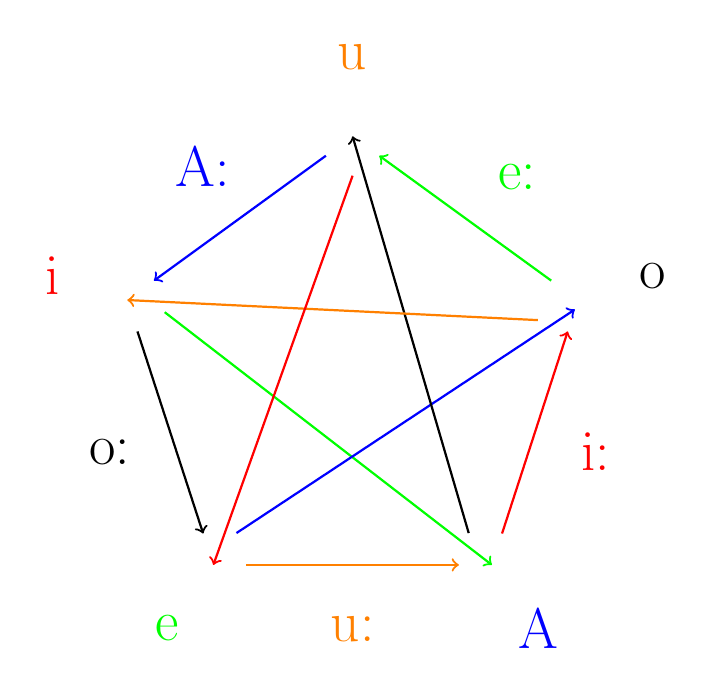
\begin{tikzpicture}

\node[regular polygon, minimum size = 8cm] (p) at (0,0) {};
\node[regular polygon, minimum size = 6cm] (q) at (0,0) {};
\node[regular polygon, minimum size = 5cm] (r) at (0,0) {};

\huge

\node[red] at (p.162){ i};
\node[orange] at (p.90) {u};
\node[green] at (p.234){e};
\node[blue] at (p.306) {\textipa{A}};
\node[black] at (p.378){o};

\node[blue] at (p.126){ \textipa{A:}};
\node[black] at (p.198){ \textipa{o:}};
\node[orange] at (p.270){ \textipa{u:}};
\node[red] at (p.342){ \textipa{i:}};
\node[green] at (p.50){ \textipa{e:}};

\draw[green, thick, ->] (r.162) -- (q.306);
\draw[blue,  thick, ->] ( r.234) -- (q.376);
\draw[black, thick, ->] (r.306) -- (q.90);
\draw[orange, thick, ->] (r.376) -- (q.162);
\draw[ red, thick, ->] (r.90) -- (q.234);

\draw[blue, thick, ->] (q.97) -- (q.155);
\draw[black, thick, ->] (q.169) -- (q.227);
\draw[orange, thick, ->] (q.241) -- (q.299);
\draw[red, thick, ->] (q.313) -- (q.371);
\draw[green, thick, ->] (q.385) -- (q.83);





\end{tikzpicture}
\end{center}

\end{document}
